\documentclass[12pt]{iopart}
\usepackage{iopams}  
\usepackage{braket}
\usepackage{graphicx}
\usepackage{subfigure}
\usepackage{cite}
\usepackage{algorithm}
\usepackage{algorithmic}



\begin{document}
\newcommand{\swave}[0]{$\it{s}$-wave }
\newcommand{\pwave}[0]{$\it{p}$-wave }
\newcommand{\K}{ $^{40}\rm{K}$}
\newcommand{\Rb}{ $^{87}\rm{Rb}$}
\newcommand{\us}{$\mu \rm{s}$} 
\newcommand{\mT}{$m\rm{T}$}

\title[]{Direct observation of Feshbach enhanced \swave scattering of fermions}

\author{D Genkina$^1$, LM Aycock$^{1,2}$, BK Stuhl$^1$, H-I Lu$^1$ and IB Spielman
$^1$\footnote{Corresponding author}}

\address{$^1$Joint Quantum Institute, National Institute of Standards and Technology, and University of Maryland, Gaithersburg, MD, 20899 USA}
\address{$^2$Physics Department, Cornell University, Ithaca, NY 14850 USA}

\ead{ian.spielman@nist.gov}

\begin{abstract}
We directly measured the \swave{} scattering cross-section of \K{} atoms accross a Feshbach resonance. We collided a pair of degenerate clouds and imaged the scattered atoms. Owing to their low density, few atoms scattered, even near the resonance. To optimize signal to noise, we develop techniques to interpret absorption imaging in the regime where the optical intensity changes dramatically as light traverses the cloud, and recoil induced 
detuning corrections are significant. We applied these techniques to our \swave{} scattering data and extracted the resonant magnetic
field value. These imaging techniques are generally applicable, and can be used to observe effective \pwave{} scattering in the presence of spin-orbit coupling in a spin polarized  Fermi gas.

\end{abstract}

\vspace{2pc}
\noindent{\it Keywords}: Quantum gases, Atomic physics

\maketitle

\section{Introduction}
Feshbach resonances are a stand-by technique for tuning the interaction strength in ultracold atomic gases. Even weak interactions play a crucial role in the physics of atomic Bose-Einstein Condensates (BECs), giving rise to, for example, their characteristic Thomas-Fermi density profiles. The effects of interactions in Fermi gases, however, are harder to observe. The density of Fermi clouds is typically reduced by a factor of $~10^3$ from that of BECs, making it necessary to enhance the strength of interactions in order to observe them. Feshbach resonances alter the inter-atomic scattering length via the magnetic field. Not only do they enable detection of interactions, but they make it possible to tune interactions from attractive to repulsive, allowing for the phase transition from the BCS to BEC regime at sufficiently low temperatures \cite{RegalThesis}. 
\par A Feshbach resonance occurs when a bound molecular state of few atoms energetically approaches the free atomic state \cite{Chin10}. The relative energy of the free atomic states and the molecular state is defined a bias magnetic field. The Feshbach resonance can thus be approached by changing the bias field. The effect of the resonance on the scattering length between two free atoms in the appropriate hyperfine states is
\begin{equation}
a(B)=a_{bg}\left(1-\frac{\Delta}{B-B_0}\right),
\label{feshbachEq}
\end{equation}
where $a$ is the scattering length, $a_{bg}$ is the scattering length away from the resonance, $\Delta$ is the width of the resonance, and $B_0$ is the field value at which the resonance occurs. Note that the scattering length tends to infinity from either side of the resonance.
\par To use Feshbach resonances as a tool it  is necessary to have a good measurement of the parameters in the above equation.  The exact value of the resonant field value $B_0$ is impossible to calculate analytically and must be estimated via numerical models \cite{Lysebo09, Gao11} or determined experimentally \cite{Inouye98, Cornish00}. Some experimental techniques that have been used to characterize Feshbach resonances include: the observation of loss due to three-body inelastic scattering, re-thermalization timescales, or anisotropic expansion, all of which infer the elastic scattering cross section from collective behavior of the cloud \cite{Regal03,OHara02,Monroe93}. 
\par Here we present a new technique for measuring the location and width of a Feshbach resonance. We collide a pair of ultra-cold Fermi gases and directly image the resulting \swave scattering halo as a function magnetic field strength. This allows us to observe the enhancement in scattering without relying on proxy effects. We measured the fraction of atoms scattered during the collision, and from this fraction deduced the resonant magnetic field  and width of the resonance.
%\par The techniques developed in this experiment for observing Fermion scattering can be extended to engineering higher order partial wave interactions, as has been done for bosons \cite{Williams2012}.
\par Our Fermi gases are so dilute that even with the resonant enhancement of the scattering cross section, only a small fraction of the atoms scatter. This makes direct detection of \swave scattering halos difficult due to detection uncertainty, which disproportionately affects regions of low atomic density. To optimize the signal to noise for low atom numbers, we utilized a non standard imaging regime. In this regime, simulation was necessary for an accurate interpretation of the images. We performed these simulations and used the results to extract the atom number and the scattered fraction from our images.
\par This paper is in two parts. In the first, we study absorption imaging in the presence of significant time-dependent Doppler shift and show how we use our results to interpret data. In the second, we describe our\swave scattering experiment and extract a measure of the location of the Feshbach resonance in \K{}. 

\section{Absorption imaging in the presence of strong recoil induced detuning}
Every experiment requires a detection scheme. In ultracold atomic experiments, most measurements are based on interacting laser light with the atomic cloud. In our experments we used absorption imaging, the most commonly used technique. Absorption imaging relies on optical transitions between the ground and some selected excited atomic states. Such atomic transitions have an energy difference $E_0$ with an associated frequency $\omega_0 = E_0/\hbar$, and a natural transition linewidth $\Gamma$. When interacting with a laser light field an atom will scatter photons: it will absorb a photon from the light field and move up to its excited state, and then re-emit the photon in a random direction and decay back to its ground state. The  rate at which this scattering occurs is
\begin{equation}
\gamma_{sc}= \frac{\Gamma}{2} \frac{I/I_{\rm{sat}}}{1+(2\delta/\Gamma)^2 +I/I_{\rm{sat}}}, 
\label{eq:scatrate}
\end{equation}
where $I/I_{\rm{sat}}$ is the laser intensity as a fraction of the saturation intensity, and $\delta$ is the detuning, the difference between the resonant transition frequency $\omega_0$ and the frequency of the laser light $\omega_L$.  
\par An absorption image is obtained by shining an on or near resonant probe beam ($\delta\approx0$) onto the atomic cloud. Some of the light is scattered by the atoms, and the part of the beam that made it through the cloud, $I_f(x,y)$ is imaged onto a camera, as seen in Fig. \ref{fig:absorptionIntor}a (top). After the atoms leave the imaging volume, the probe light is reapplied to calibrate the intensity $I_0(x,y)$ of light unaffected by the atoms (bottom). 
\begin{figure}
	\subfigure[]{\includegraphics*[scale=0.55]{Picture1a}}
	\subfigure[]{\includegraphics*{Picture1c.pdf}}
	\subfigure[]{\includegraphics*[scale=0.55]{Picture1b}}
\caption{Absorption imaging. a. Near resonant probe light illuminates the atoms, and the transmitted light (containing a shadow of the atoms) is imaged on the camera. After the atoms depart an image of just the probe light is taken. b.  The probe beam is partially absorbed as it traverses the cloud, and the intensity seen by atoms further along the imaging direction $z$ is lowered.  c. An atomic cloud illuminated by a probe light field absorbs photons from the probe and re-emits them in all directions. This process results in a net velocity of the cloud in the direction of the probe light as well as diffusive spreading in the transverse directions.  }  
\label{fig:absorptionIntor}
\end{figure}
\par These intensities are related to the number of atoms the light encountered. Consider the light as it travels along the imaging axis $e_z$ through a 3-D atomic density profile $\rho(x,y,z)$. For the purposes of this discussion, let us focus on a single pixel of the camera, and thus a single value of $I_0$ and $I_f$ and a single column of atoms, $\rho(z)$. We will not be able to infer the entire atomic distribution, but for each pixel we can obtains the integrated density, $n = \int \rho\left(z\right) \,\mathrm{d}z$. As the light travels through a column of atoms, each atom will scatter light according to Eq. (\ref{eq:scatrate}). Therefore, the atoms further along the imaging axis $z$ will experience a reduced optical intensity, as seen in Fig. \ref{fig:absorptionIntor}b. On resonance ($\delta=0$), the intensity change from scattering as a function of $z$ is
\begin{equation}
\frac{dI(z)}{dz}=\hbar\omega_L\rho\gamma_{sc}=-\rho\sigma_0\frac{I(z)}{1+I(z)/I_{\rm{sat}}},
\end{equation}
where $\sigma_0$ is the resonant scattering cross section. 
 This equation can be easily integrated to obtain  \cite{Reinaudi07}
\begin{equation} 
\sigma_0 n = -\ln\left(\frac{I_f}{I_0}\right) + \frac{I_0-I_f}{I_{\rm{sat}}}.
\label{eq2}
\end{equation}
In the limit where the probe intensity is much smaller than the saturation intensity, $I_0\ll I_{\rm{sat}}$, this reduces to $-\ln \left(I_f/I_0\right)$: optical depth, or $OD$. Since this is the simplest possible model that relates the observed intensities to the column density $n$, we call this quantity $OD_0$. When the probe intensity is comparable to the saturation intensity, the second term in Eq. (\ref{eq2}) becomes significant, and we define the optical density corrected for high probe intensity, or
\begin{equation} 
OD_1 = OD_0 + \frac{I_0-I_f}{I_{\rm{sat}}}.
\label{eq:OD1}
\end{equation}
There are further corrections that this equation does not take into account. In particular, it neglects the atomic recoil momentum and its effect on the laser detuning, which will be discussed below.
\par When an atom absorbs a photon from the laser light field and is excited to a higher energy level, by conservation of momentum it must also acquire a velocity in the direction of the light field. This recoil velocity is given by $v_r=\hbar k/m$, where $k=2\pi/\lambda$ is the wavenumber of the light field with wavelength $\lambda$ and $m$ is the atomic mass. When the atom returns to its ground state, the photon is re-emitted with some momentum $\vec{p}_e$. Over many photons, this momentum distribution averages to zero, $\int\vec{p}_e\mathrm{d}^3 x=0$.  The variance, however, is not zero, allowing the atoms to acquire some momentum transverse to the laser field. We will ignore this correction, but the effect of this on the atomic cloud is picture in Fig. \ref{fig:absorptionIntor}c. 
\par Once the atoms absorb enough photons that they acquire a substantial velocity in the direction of the light field, this velocity Doppler shift them from resonance with the light field. After scattering $N$ photons an atom acquires an average velocity $N v_r$ and an additional detuning $\delta=k N v_r$. Therefore, even if the probe beam is initially on resonance with the atomic transition, we cannot neglect the detuning term in the scattering rate as time goes on. Furthermore, this detuning varies both with imaging time $t$ and with distance along the propagation direction $z$ (Fig. \ref{fig:detunedBlobs}). Thus, the intensity lost to the atoms also acquires a time dependence: 
\begin{equation}
\frac{dI(t,z)}{dz}=\sigma_0 \rho \frac{I(t,z)}{1+[2\delta(t,z)/\Gamma]^2 +I(t,z)/I_{\rm{sat}}}, \label{eq3}
\end{equation}
where the detuning $\delta$ is
\begin{equation}
\delta(t,z)=\frac{v_r}{\hbar c \rho}\int_0^t \frac{dI(z,\tau)}{dz}\,\mathrm{d}\tau; \label{eq4} 
\end{equation}
the relationship between the atomic density and the observed intensities is no longer straightforward.
\begin{figure}
	\includegraphics*{Figure1.pdf}
\caption{Dependence of velocity and detuning on position along the imaging axis in an atomic cloud of \K{} for three different imaging times and a probe intentisy $I_0=1.5 I_{\rm{sat}}$, as obtained by numerical simulation.}  
\label{fig:detunedBlobs}
\end{figure}
\par By considering this equation perturbatively in time we obtain corrections to second order in imaging time \cite{LJLthesis}
\begin{equation}
\sigma_0n\approx OD^{(0)}+OD^{(1)}t+OD^{(2)}t^2 = OD_2
\end{equation}
\begin{equation}
OD_2= OD_1+\frac{(kv_rt)^2}{3}\left[\frac{I_{\rm{sat}}}{I_f+I_{\rm{sat}}}-\frac{I_{\rm{sat}}}{I_0+I_{\rm{sat}}}+\mathrm{ln}\left(\frac{I_f+I_{\rm{sat}}}{I_0+I_{\rm{sat}}}\right)\right].
\label{eq:OD2}
\end{equation}
 However, as shown in  Fig. \ref{fig:ODcorrections}, the perturbative treatment breaks down shortly after the zeroth order approximation of Eq. (\ref{eq2}).To adequately correct for the recoil induced detuning of the atoms, we numerically simulated the imaging process for $I_f$ as a function of imaging time, atomic density, and probe intensity. 
\begin{figure}
	\includegraphics*{figure2.pdf}
\caption{Using time dependent $I_f$ values obtained from recoil detuning corrected simulation of on-resonant imaging of $^{40}K$ atoms at probe intensity $I_0=0.8\, I_{\rm{sat}}$, this graph shows the optical depths obtained by each model. The `true' optical depth is $\sigma_0 n=1.6$. $OD_1$ is the high probe intensity corrected optical depth given by Eq. (\ref{eq2}). $OD_2$ is the high probe intensity corrected and expanded to second order in time optical depth, Eq. (\ref{eq:OD2}) \cite{LJLthesis}. The recoil time is the time it takes for the cloud, on average, to become detuned by a linewidth $\Gamma$. Both models start to differ from the true value before a recoil time.  }  
\label{fig:ODcorrections}
\end{figure}
\par In the following, we describe two versions of this simulation. First, we take a simplistic approach where the spatial distribution of atoms does not change appreciably during the imaging time and can be treated statically. We test this approach in known limits and then check the validity of the static assumption.For realistic input parameters, this assumption is invalid. We developed a slightly more sophisticated quasi-classical approach and allowed the atoms to move during the imaging time, allowing us to simulate the phase space evolution of atoms subjected to probe light. While the atomic trajectories are wildly different than in the static atom approximation, the predicted ODs only vary on the 0.5$\%$ level between the two models. 


\subsection{Stationary atom model}
To solve Eqs. (\ref{eq3})-(\ref{eq4}), we start with a 1-d distribution distribution of atomic densities $\rho(z)$, assumed to be Gaussian in shape. We divided the cloud into spatial bins (the bin size was chosen such that decreasing the bin size further changed the result at the $10^{-5}$ level).  In this approximation, we keep the number of atoms in each bin constant.  The algorithm used is shown in Alg. [\ref{algorithm1}]. We call the optical depth obtained from this algorithm $OD_{corr1}$.

\begin{algorithm}
\caption{Stationary atom model}
\label{algorithm1}
\begin{algorithmic}
\STATE $I[n=0,t]=I_0$ \COMMENT{$n$ is the bin index, $t$ is the time index, $I$ is in units of $I_{\rm{sat}}$} 
\STATE $\delta[n, t=0]=0$ \COMMENT{light initially resonant, $\delta$ in units of $\Gamma/2$}
\STATE $I_f=0$ \COMMENT{no light has entered the cloud}
\FOR[loop over time steps]{$t=0$ to $t_f$}
 \FOR[loop over bins, N is total bin number]{$n=1$ to $N$}
 \STATE $A=\sigma_0\rho[n] dz$ \COMMENT{$dz$ is the size of spatial step}
 \STATE $B=v_r dt/(\hbar c \rho[n])$  \COMMENT{$dt$ is the size of the time step}
\STATE $I[n,t]=I[n-1,t] - A I[n-1,t]/(1+\delta[n,t-1]^2+I[n-1,t])$  \COMMENT{Eq. (\ref{eq3})}
\STATE $\delta[n,t]=\delta[n,t-1]+B\left(I[n-1,t]-I[n,t]\right)$  \COMMENT{Eq. (\ref{eq4})} 
\ENDFOR 
\STATE $I_f =I_f+ I[N,t]dt$
\ENDFOR
\STATE $OD_{corr1}=-\ln{(I_f/I_0t_f)}$
\end{algorithmic}
\end{algorithm}

\par We checked the validity of our simulation in the limits in were the problem is analytically solvable. When the probe intensity is much weaker than the saturation intensity, $I_0\ll I_{\rm{sat}}$, the atoms' velocity is hardly changed, and Eq.(\ref{eq3}) reduces to 
\begin{equation}
\frac{dI(z)}{dz}=-\rho\sigma_0 I(z),
\end{equation}
from which we recover 
\begin{equation}
\sigma_0 n = OD_0 = -\ln I_0/I_f. \label{eq6}
\end{equation}
In the limit that the probe intensity is much stronger than the saturation intensity, $I_0/I_{\rm{sat}}\gg \delta/2\Gamma$, even far detuned atoms will absorb light at their maximum, allowing us to again neglect the time dependence of the detuning. Equation (\ref{eq3}) becomes 
\begin{equation}
\frac{dI(z)}{dz}=-\rho\sigma_0 I_{\rm{sat}}, 
\end{equation}
which integrates to 
\begin{equation}
\sigma_0 n = \frac{I_0 - I_f}{I_{\rm{sat}}}. \label{eq8}
\end{equation}
We recognize the right hand sides of Eq. (\ref{eq6}) and Eq. (\ref{eq8}) as the two terms in the expression for $OD_1$ in Eq. (\ref{eq2}). Thus, as shown in  Fig. \ref{fig:IsatLimits}, in both limits $OD_{corr1}$  coincides with $OD_0$ in both the small and large probe intensity limits. 
\begin{figure}
	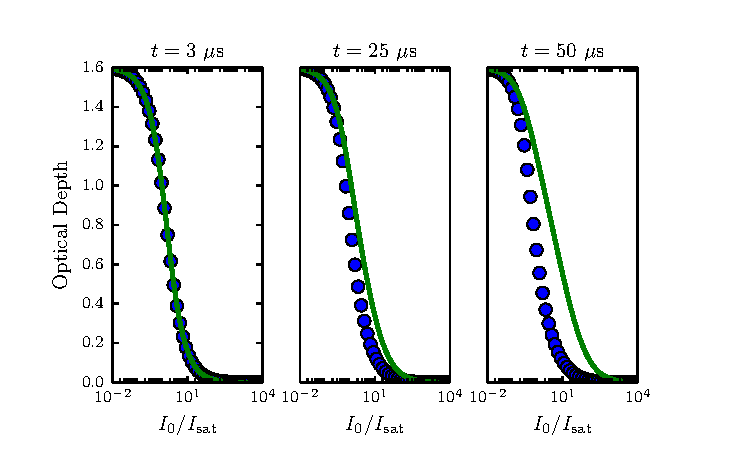
\includegraphics{figure3.pdf}
\caption{Optical depth as a function of probe intensity as predicted by the simulation (blue symbols) and by Eq. (\ref{eq6}) (green curves), for three different imaging times. The predictions agree in both the high and low intensity limits, and differ for probe intensities comparable to the saturation intensity. The difference is enhanced with increased imaging time.}  
\label{fig:IsatLimits}
\end{figure}
\par We used the results of this simulation to check if the stationary atom assumption is valid, i.e. if the distance traveled by the atoms during the imaging time is less than the bin size. As can be seen from Fig. \ref{fig:atomTravel}, not only do the atoms travel more than the bin size, but they travel far beyond the initial extent of the cloud. Moreover, owing to the high scatter rate, the back of the cloud overtakes the front for long imaging times. Thus, the atomic distribution as a function of position changes dramatically during the imaging pulse, and the stationary assumption is invalid. 
\begin{figure}
	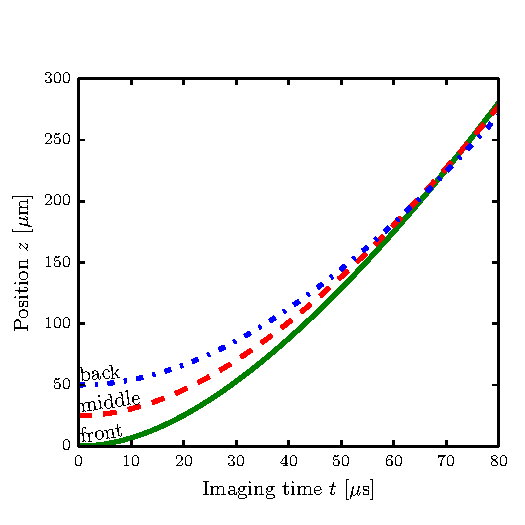
\includegraphics{figure4.pdf}
\caption{Position of atoms as a function of imaging time for atoms in the first, middle, and last bins of the simulation, obtained by integrating their velocities. The probe intensity here is $1.2 I_{\rm{sat}}$, and the optical depth is 1.6.}  
\label{fig:atomTravel}
\end{figure}

\subsection{Traveling atom model}
To account for the changing atomic distribution during the imaging pulse, we simulate the classical kinetics of atoms subject to the recoil driven optical forces. To simulate large ensembles in a reasonable time, we use "superatoms",  each describing the aggregate behavior of $N_{sa}$ atoms. The amended algorithm is shown in alg.[\ref{algorithm2}]. 
\begin{algorithm}
\caption{Travelling atom model}
\label{algorithm2}
\begin{algorithmic}
\STATE $z[n]=z_0$, $\delta[n]=0$ \COMMENT{initialize position and detuning for each superatom, labeled by index $n$}
\STATE $O[i]=n$ \COMMENT{make a list of superatom indexes, ordered by position}
\STATE $I[n=0,t]=I_0$ \COMMENT{ $t$ is the time index, $I$ is in units of $I_{\rm{sat}}$} 
\STATE $I_f=0$
\FOR[loop over time steps]{$t=0$ to $t_f$}
 \FOR[loop over superatoms]{$i=1$ to $N$}
\STATE $n=O[i]$ \COMMENT{apply probe intensity to superatoms in order of appearance}
 \STATE $A=\sigma_0 N_{sa} dz$ \COMMENT{dz is length over which atoms were grouped into single superatom}
 \STATE $B=v_r dt/(\hbar c  N_{sa})$  \COMMENT{dt is the time step}
\STATE $I[n,t]=I[n-1,t] - A I[n-1,t]/(1+\delta[n]^2+I[n-1,t])$  \COMMENT{Eq. (\ref{eq3})}
\STATE $\delta[n]\mathrel{+}=B\left(I[n-1,t]-I[n,t]\right)$  \COMMENT{Eq. (\ref{eq4}), detuning in units of $\Gamma/2$} 
\STATE $z[n]\mathrel{+}=dt\Gamma\delta/2k$ \COMMENT{$k$ is the wavenumber, $\Gamma\delta/2k$ is the velocity at $\delta$ detuning}
\ENDFOR 
\STATE $O[i]$=sort($n$, key =$z[n]$) \COMMENT{sort superatoms indexes by current position}
\STATE $I_f  \mathrel{+}= I[N,t]dt$
\ENDFOR
\STATE $OD_{corr2}=-\ln{(I_f/I_0t_f)}$
\end{algorithmic}
\end{algorithm}
\par First, we check the velocity predicted in this model against known limits. One such limit is that of a single superatom. In this case, there is no attenuation, and the intensity seen by the superatom is constant at $I_0$. Only the detuning of the single superatom evolves in time, and Eqs. (\ref{eq3}) and (\ref{eq4}) give
\begin{equation}
\frac{dD(t)}{dt}= k_R v_r \frac{\tilde{I}}{1+D^2+\tilde{I}},
\label{eq10}
\end{equation}
where $D = 2\delta/\Gamma$, and $\tilde{I} = I_0/I_{\rm{sat}}$. Equation (\ref{eq10}) can be solved numerically, and is in good agreement with our simulation, as seen in Fig. \ref{fig:oneAtomVel}.
\begin{figure}
	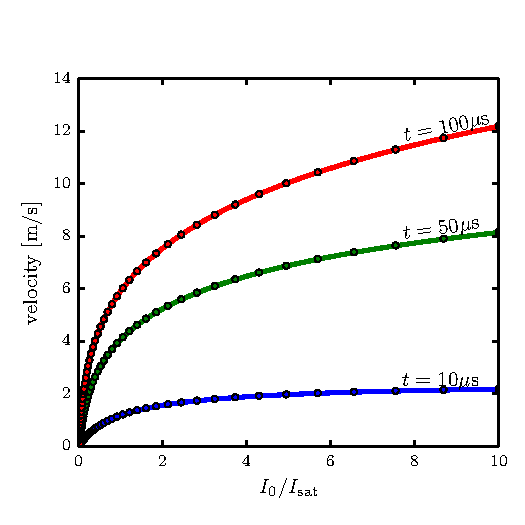
\includegraphics{figure5.pdf}
\caption{The velocity of a single superatom as a function of probe intensity for various imaging times. Simulation data (dots) and analytical solutions (lines) are in good agreement.}  
\label{fig:oneAtomVel}
\end{figure}
\par We use this model to study the time evolution of the cloud shape during imaging and visualized the phase space evolution of superatoms, shown in Fig. \ref{fig:phaseSpace}. The cloud shape is strongly distorted during the imaging time. 
\begin{figure}
	\subfigure[]{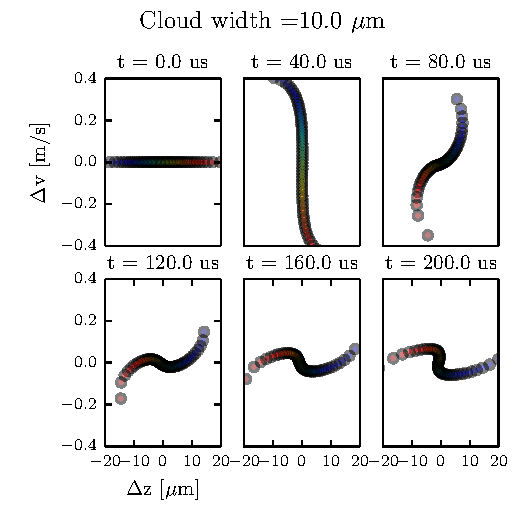
\includegraphics{figure6a.pdf}}
	\subfigure[]{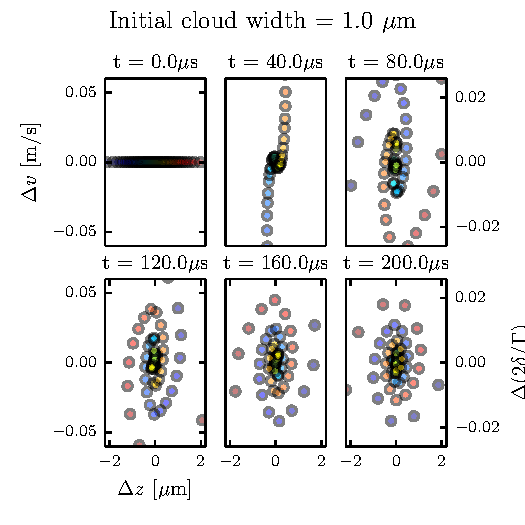
\includegraphics{figure6b.pdf}}
\caption{Phase space evolution of an atomic cloud exposed to probe light with intensity $I_0=1.2 I_{\rm{sat}}$. We defined $\Delta v=v -\left< v(t) \right>$  and $\Delta z=z-\left< z(t) \right>$, subtracting out the center of mass position and velocity of the cloud. The optical depth is 1.6, and the initial cloud is a gaussian with a width of 10 $\mu$m in (a) and 1 $\mu$m in (b).}  
\label{fig:phaseSpace}
\end{figure}
\par We compare the optical depths predicted by each of the two models, $OD_{corr1}$ and $OD_{corr2}$, and, as seen Fig. \ref{fig:atomTravel}, the predicted optical depths are hardly changed by including the full time evolution:  $\left|OD_{corr1}-OD_{corr2}\right|/OD_{corr1} \le 0.005$. Thus, for the purposes of deducing the atom density from experimental optical depths,the stationary atom model is sufficient. Furthermore, we simulated a range of initial density profiles $\rho(z)$, and found their impact to be negligible - the only observable is the integrated atomic density $n=\int\rho(z)\mathrm{d}z$. 
\begin{figure}
	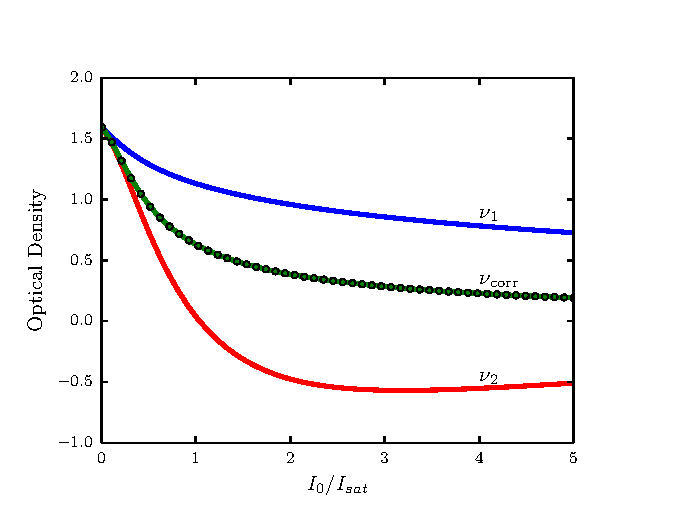
\includegraphics{figure7.pdf}
\caption{Optical depth as a function of probe intensity for an imaging time $t=100$ \us. The two versions of simulated optical depth, $OD_{corr1}$ (green curve) and $OD_{corr2}$ (green dots) are virtually indistinguishable. }  
\label{fig:atomTravel}
\end{figure}

\subsection{Signal to noise optimization}
This simulation allows us to interpret experimentally obtained initial and final intensities. For a given imaging time, we create a look-up table of predicted optical depth as a function of probe intensity and atomic density. We then find the observed optical depth on this table, with the given probe intensity, and infer the atomic density. The uncertainty in the measured intensities can be propagated through this procedure, and we establish optimal imaging parameters to maximize the signal to noise ratio of this detection scheme. 
\par Here, the only source of measurement uncertainty we consider is the Poisson distributed photon shot noise, with a standard deviation proportional to $\sqrt{N_p}$, where $N_p$ is the photon number. We then propagate this uncertainty through our correction scheme to obtain the uncertainty in our deduced value of $\sigma_0 n$. We define the signal to noise ratio (SNR) as $\sigma_0 n/\delta_{\sigma_0 n}$, where $ \delta_{\sigma_0 n}$ is the propagated measurement uncertainty.
\par As seen in Fig. \ref{fig:SNR}a, after about 40\us{} extending the imaging time no longer yields appreciable improvement in signal to noise ratio. Imaging for 40\us{} as opposed to 10\us{} where the uncorrected model is appropriate, improves the SNR by a factor of  1.5. We performed the experiments described in the second section at 40\us{} imaging time. Figure \ref{fig:SNR}b shows that the optimal probe intensity varies with the magnitude of $OD$s. For low atom numbers, $OD\approx0.1$, a probe intensity of $I_0\approx0.6I_{\rm{sat}}$ is best. However, in our experiment the probe intensity had a gaussian profile and is not uniform over the whole image.  The typical probe intensities used in our experiments were in the $I_0=0.1I_{\rm{sat}}-0.7I_{\rm{sat}}$  range.
\begin{figure}
	\subfigure[]{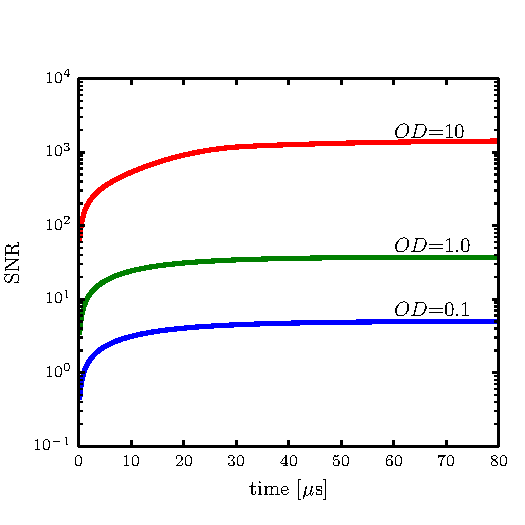
\includegraphics{figure9a.pdf}}
	\subfigure[]{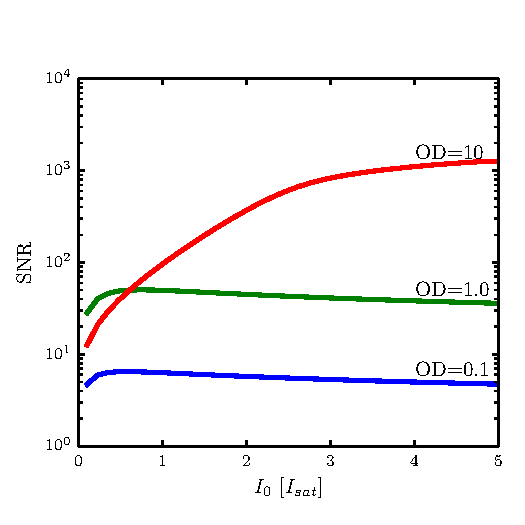
\includegraphics{figure9b.pdf}}
\caption{Signal to noise ratio (SNR) for three different optical depths after correcting for recoil induced detuning. (a) SNR as a function of probe intensity $I_0/I_{\rm{sat}}=5.0$ and (b) SNR as a function of probe intensity for an imaging time of 50 \us{}.}  
\label{fig:SNR}
\end{figure}

\subsection{Calibration of saturation intensity}
A key component of good detection is a well calibrated measurement apparatus. In this case, the measurement apparatus is a CCD camera used to take the absorption images.  Each camera pixel  converts the photons it is exposed to, with some efficiency, into photoelectrons, and then to a digital signal: and integer we  call  `counts'. The number of photons that hit a pixel is proportional to the number of `counts' it outputs. However, the proportionality constant depends o many factors, such as the quantum efficiency of the camera, the electronic gain during the readout process, and the polarization of the probe light. 
\par We determined this factor through direct experiment. In the limit where the system is adequately described by Eq. (\ref{eq6}), only the ratio of the initial and final intensities matter, and this proportionality constant is irrelevant. In all other regimes, however, the ratio of the initial and final intensities to the saturation intensity also comes into play, making the proportionality constant significant. One way to approach this calibration is to determine the value of the saturation intensity in `counts' per unit time. 
\par To calibrate the saturation intensity in camera counts per unit time, we take absorption images of a cloud of \K{} atoms at three different imaging times, 40 \us{}, 100 \us{}, and 200 \us{}, at varying probe intensities. We pick a small square in the center of the cloud, where the atomic density is approximately uniform, and average the initial and final intensities of each pixel in the square. Thus, for each image we obtain $I_0$ and $I_f$, in counts per microsecond. We then do a least squares fit of $OD_{corr}$, our simulated optical depth, to the data. The two fit parameters are the atomic density $n$ at the center of the cloud and the value of $I_{\rm{sat}}$ in counts per microsecond. As seen in Fig. \ref{fig:isatCalib}, the model produces a good fit to the experimental data, and we obtain a calibration of the saturation intensity for our experiment. 
\begin{figure}
	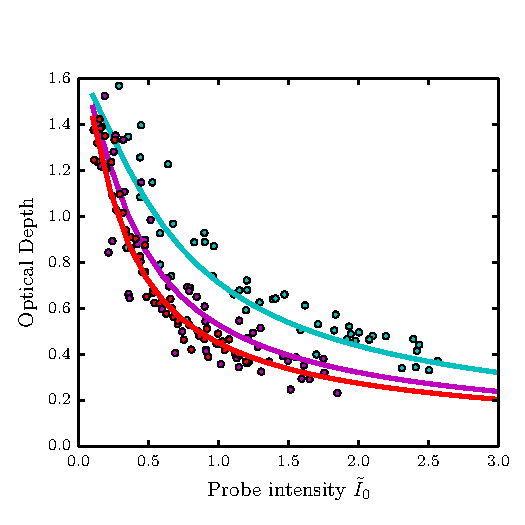
\includegraphics{figure8.pdf}
\caption{The optical depth as a function of probe intensity for three imaging times: $t=40$\us{} (blue),  $t=75$\us{} (green),  $t=100$\us{} (red). The dots represent experimental data and the lines represent the best fit of simulated data. The optimal fit parameters pictured are a $\sigma_0 n$ of 1.62 and saturation intensity of 29 counts/\us{}. }  
\label{fig:isatCalib}
\end{figure}


\section{S-wave scattering experiment}
In this section we describe our Fermi scattering experiment. We scattered two counter-propagating \K{} clouds and observed the resulting \swave{} halo of scattered atoms.  We measured the dependence of the scattered atomic fraction on the bias magnetic field in the vicinity of the Feshbach resonance. We used this data to extract the location of the magnetic fields resonance of 20.247(2)  \mT{} and a width of 1.0(1)  \mT{}.
\subsection{Experimental procedure}
We prepared clouds of cold \K{} atoms in a hybrid \K{} and \Rb{} apparatus. We used a Zeeman slower to slow both species before being captured in a magneto-optical trap (MOT) allowed both species to cool in optical molasses for 2 miliseconds. We optically pumped both species into a magnetically trappable state, $\ket{F=9/2, m_F=9/2}$ for \K{} and $\ket{F=2,m_F=2}$ for \Rb{}. Both species were then loaded into a quadrupole magnetic trap, and cooled evaporatively. Since the \K{} atoms are dilute and only interact very weakly with each other, they re-thermalize primarily due to interaction with \Rb{} atoms, and therefore the \Rb{} atoms are necessary to evaporatively cool \K{}. We then load the atoms into a crossed optical dipole trap, with trap frequencies of $(\omega_x/2\pi,\omega_y/2\pi,\omega_z/2\pi) =(39, 42, 124)$ in the three spatial directions. We continued evaporative cooling by slowly ramping down the dipole trap. We then used adiabatic rapid passage (ARP) to transfer the \Rb{} atoms from the $\ket{F=2, m_F=2}$ state to the  $\ket{F=1, m_F=-1}$ absolute ground state. This state was chosen to minimize spin changing collisions with \K{} atoms during any further evaporation.  We then briefly applied an on-resonant probe laser, ejecting any remaining \Rb{} atoms in the $F=2$ manifold from the trap. We again used ARP to transfer the \K{} atoms into an equal superposition of $\ket{F=9/2,m_F=-9/2}$ and $\ket{F=9/2,m_F=-7/2}$, and further evaporated in the dipole trap. Since \Rb{} is heavier than \K{}, we were able to evaporate the \K{} atoms past the point where \Rb{} atoms were no longer suspended against gravity and fell out of the trap.  These hyperfine states of \K{} were then used to study their Feshbach resonance. 

\par We ramped the bias field in a two-step fashion to the desired value $B$ near the Feshbach resonance. We approached the field using a large pair of  coils in Helmholtz configuration to bring the magnetic field 0.59 \mT{} of $B$. We held the atoms at this field for 100 $m\rm{s}$ to allow the eddy currents induced by the large coils to settle, and then used a smaller set of Helmholtz coils to hop the field the remaining 0.59 \mT{}. We took two sets of data: one approaching the resonance from below, where we hopped the large coils to $B-0.59 \mT{}$ and used the small coils to hop up to the desired field, and one coming from above the resonance, where we hopped the large coils to  $B+0.59  \mT{}$ and then used the small coils to hop the field down to the desired value. This allowed us study the resonance from both sides without the added losses associated with going through the resonance \cite{Chin10}.
\par The magnetic field $B$ was independently calibrated by pusling on a pre-set radio frequency signal and finding the large coil current setting that optimally transferred \K{} atoms in $\ket{F=9/2,m_F=-9/2}$ to an equal superposition of $\ket{F=9/2,m_F=-9/2}$ and $\ket{F=9/2,m_F=-7/2}$ via jitter in the small coils causing decoherence.
\par Once we had the Fermi cloud at the intended bias field, wesplit the cloud into two spatially overlapping components with momenta $p=\pm 2\hbar k_L$  and observed scattering as they moved through each other and separated. To create these counterpropagating components, we used a double pulse sequence \cite{Wu05} of a near resonant 1-d retro-reflected optical lattice. The pulse sequence was optimized to transfer most of the atoms into the $\pm 2 \hbar k_L$ momentum states, where $k_L$ is the recoil momentum of the lattice. Since the initial Fermi gas had a wide momentum spread (in contrast to a BEC, which has a very narrow momentum spread), and the lattice pulsing is a momentum dependent process, not all the atoms were successfully transferred into the target momentum states. We optimized our pulse times to minimize the atoms remaining in the zero momentum state. The optimized pulse times were 23 \us{} for the first square pulse, 13 \us{} off interval, and 12 \us{} for the second square pulse. An 8$E_L$ lattice was used, where $E_L=\hbar^2 k_L^2/2m_K$ is the lattice recoil energy.  
\par We then released the atoms from the trap and allowed 1ms for the two opposite momentum states within the cloud to pass through each other, scattering on the way. For the data taken coming from below the Feshbach resonance, we then simply ramped down the field and imaged the atoms. For the data taken coming from above the Feshbach resonance, we ramped the field back up, retreating through the resonance if it had been crossed, recovering any molecules that were created, and then quickly hopped the field back down and imaged the atoms. We use a 40 \us{} imaging pulse with $I_0/I_{\rm{sat}}\approx 0.6$ at the center. 
\par The total time-of-flight, time from the moment the atoms were released from the trap to when they were imaged, was $t_{TOF}=6.8$ $m\rm{s}$. In such an image, observed atomic position is determined by the distance traveled during $t_{TOF}$, which is determined by its initial velocity when it was released from the trap. Therefore, this technique measures the momentum and not the position distribution of the atoms. 
\subsection{Methods}
\par We first corrected each image for recoil induced detuning as described in the previous section. An example of this correction procedure is shown in Fig. \ref{fig:SampleCorrection}.  To improve the signal and compensate for our shot to shot number fluctuations, we took 15 nominally identical images for each data point and, after correcting, averaged them.
\begin{figure}
	\subfigure[]{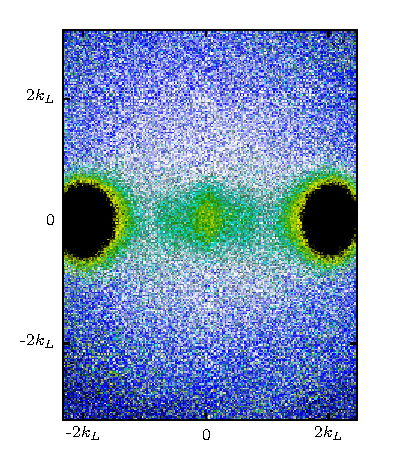
\includegraphics{figure10a.pdf}}
	\subfigure[]{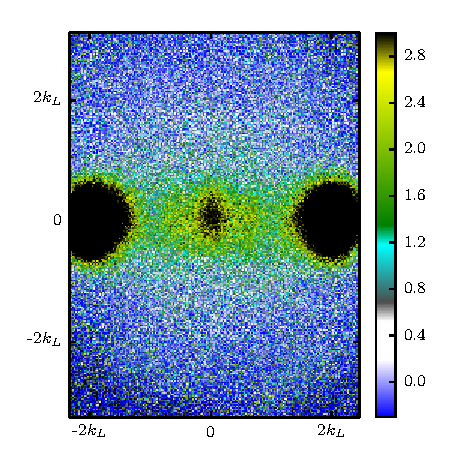
\includegraphics{figure10b.pdf}}
\caption{An example of our absorption image after 6.8 $m$s time of flight. The 1-D lattice imparts momentum along $e_x$. The two large clouds on the left and right are the atoms in the $\pm 2k_r$ momentum orders that passed through each other unscattered. The smaller cloud in the center is the atoms that remained in the lowest band of the lattice after pulsing, and thus obtained no momentum. The thin spread of atoms around these clouds is the atoms that underwent scattering.   This image was taken coming from below the Feshbach resonance at 20.07  \mT{}. (a) Raw optical depth, (b) corrected optical depth.}  
\label{fig:SampleCorrection}
\end{figure}
\par We extracted the fraction of atoms that underwent a single scattering event as a function of the bias field. An atom that underwent a single scattering event is easily identified, as two atoms that scatter elastically keep the same amplitude of momentum, but align along an arbitrary direction. Therefore, an atom traveling at $2 \hbar k_L$ to the right that collides with an atom traveling at $2 \hbar k_L$ to the left will depart with a momentum of $2 \hbar k_L$ in some direction, and in a time of flight image such atoms will lie in a spherical shell centered on the center of mass, giving the scattering halo, pictured in Fig. \ref{fig:halo}a. 
\begin{figure}
	\subfigure[]{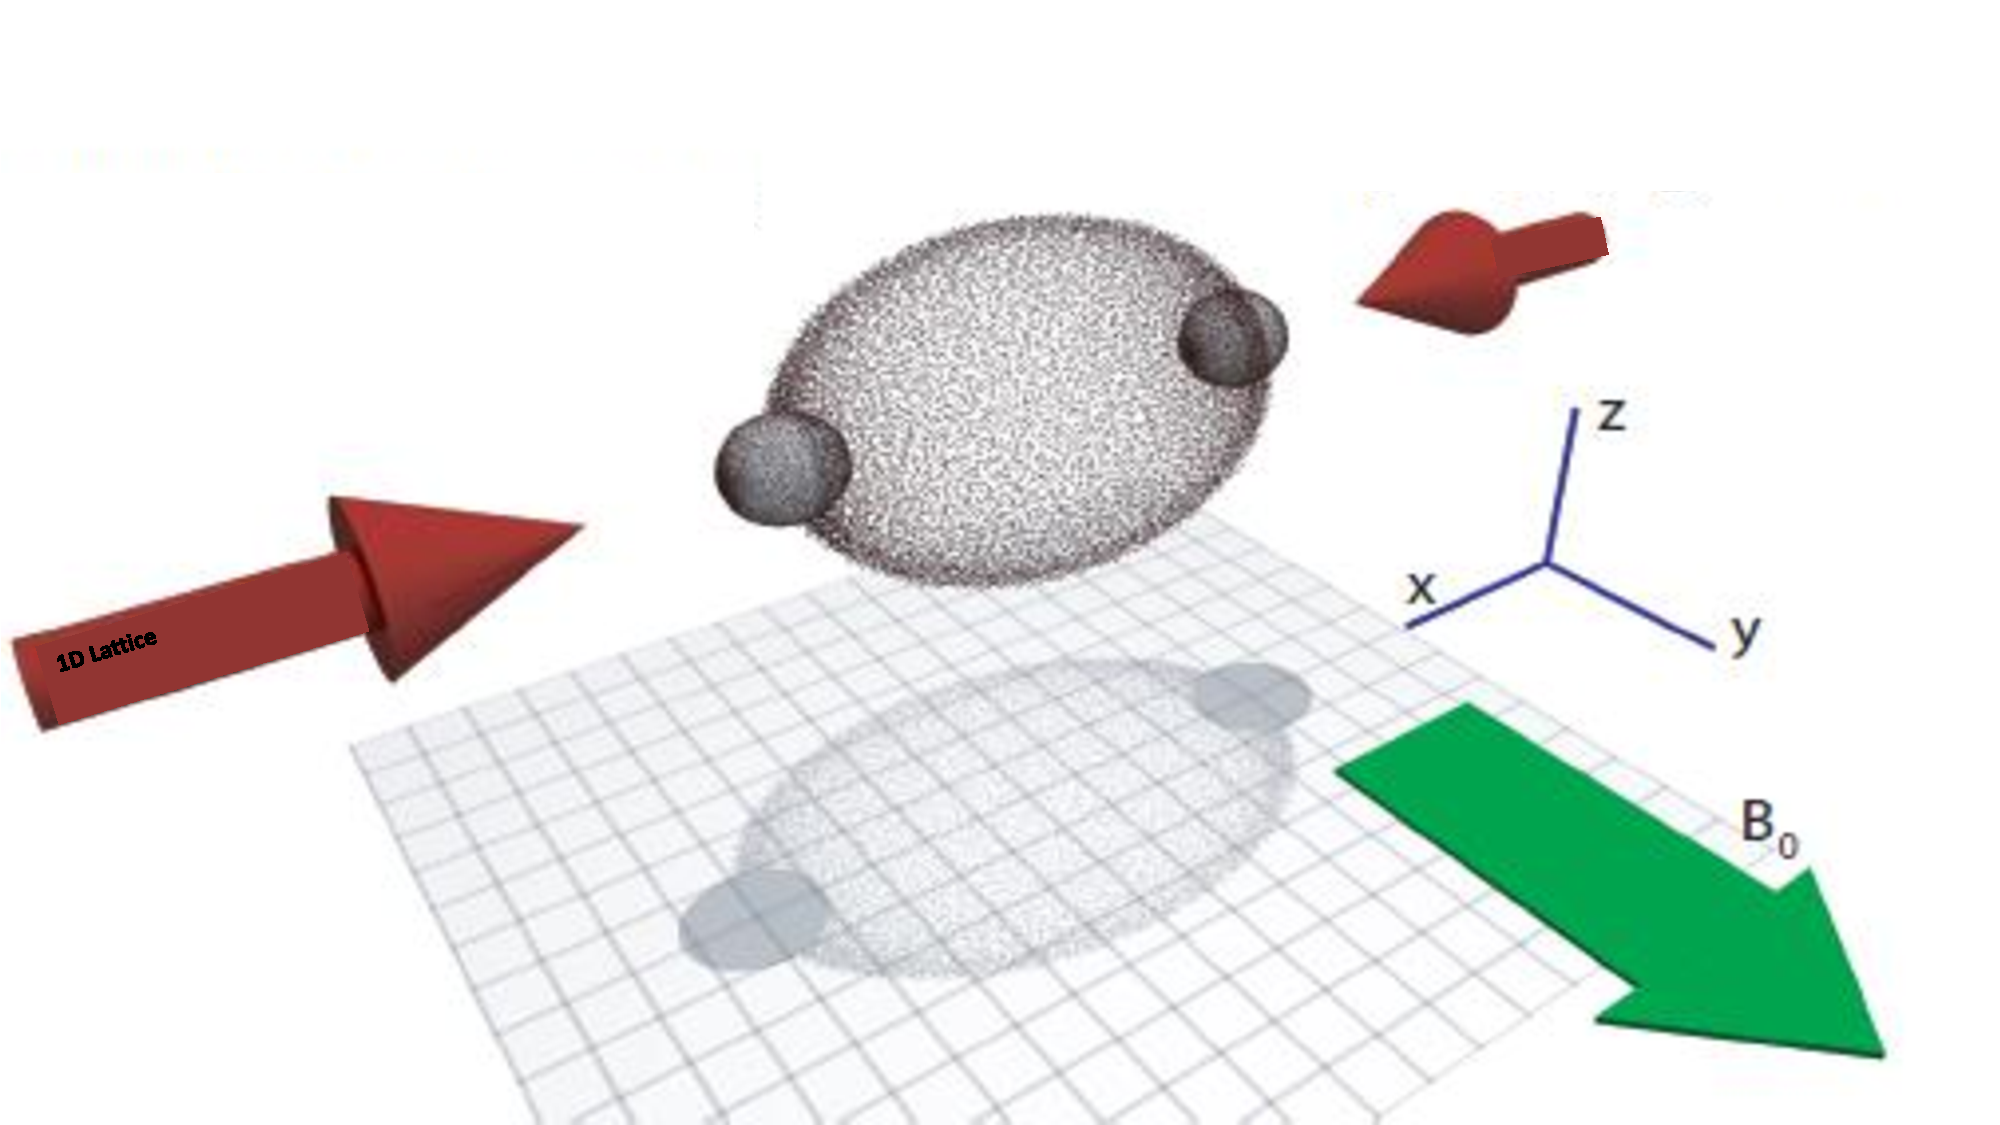
\includegraphics[scale=0.075]{Picture12.pdf}}
	\subfigure[]{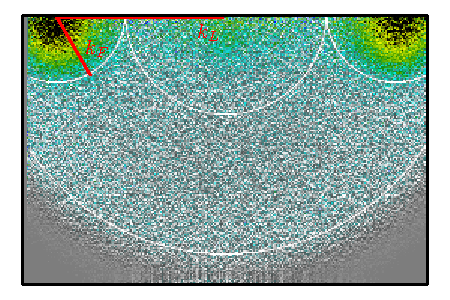
\includegraphics{figure12b.pdf}}
\caption{(a) Our experimental setup. After time of flight, the two clouds traveling along $\pm e_x$ directions have separated and the atoms that underwent a single scattering event were evenly distributed in a scattering halo around the unscattered clouds. The 1D lattice defined the axis of cylindrical symmetry. (b) Inverse Abel transformed image. The atoms within the Fermi momentum $k_F$ of each unscattered cloud center are in the unscattered region and counted towards the total unscattered number. The atoms outside the radius $k_r-k_F$ but inside $k_r+k_F$ but outside the unscattered region are counted towards the number of single scattered atoms.   }  
\label{fig:halo}
\end{figure}
\par Absorption images captured the integrated column density along $e_z$, a projected 2-d atomic distribution. To extract the radial dependence of the 3-d distribution from the 2-d image, we performed a standard inverse Abel transform. The inverse Abel transform assumes cylindrical symmetry, which was present in our case, with the axis of symmetry along $e_x$, defined by the lattice. We thus obtained the atomic distribution as a function of $r$, the radial distance from the scattering center, and $\theta$, the angle between $r$ and symmetry axis $e_x$, integrated over $\phi$, the azimuthal angle around the $x$ axis. 
\par We then extracted the number of scattered atoms $N_{scat}$, as a fraction of the total atom number $N_{tot}$, for each bias magnetic field, as shown in Fig. \ref{fig:halo}b. We obtained the unscattered atom number by counting the number of atoms in the two unscattered clouds. We obtained the number of atoms that underwent a single scattering event by counting the number of atoms outside the Fermi radius of the unscattered clouds, but inside the arc created by rotating the Fermi momentum $k_F$ around the original center of the cloud (white arcs in Fig. \ref{fig:halo}b). The total atom number in the image was the sum of those two.
\par We then used our data to deduce the resonant field value $B_0$ and width of the resonance  $\Delta$, the parameters in Eq. (\ref{feshbachEq}).  Since we were in the low energy regime, the scattering cross-section was given by $\sigma=4\pi a^2$. 
\par One way to think about the scattering cross-section $\sigma$ is that the probability $P_{scat}$ that a single particle will get scattered when incident on a cloud of atoms with a surface density of $N/A$ is given by $P_{scat}=\sigma N/A$. In our case, half the initial cloud, with atoms number $N_{tot}/2$, is incident on the other half of the initial cloud, again with $N_{tot}/2$ atoms. Thus, the number of scattered atoms should be given by $N_{scat}= (N_{tot}/2) \sigma  (N_{tot}/2)=\sigma N_{tot}^2/4A$, where $A$ is the cross-sectional area of the cloud. Assuming $A$ is constant for all our data, we can absorb the factor of 4A into our definition of $a_{bg}$, along with the $4\pi$, to obtain the fit function
\begin{equation}
\frac{N_{scat}}{N_{tot}^2}=\tilde{a}_{bg}^2\left(1-\frac{\Delta}{B-B_0}\right)^2 + C.
\label{eq:fit}
\end{equation}
\par We found that our imaging noise skewed towards the positive, giving rise to a small background offset. We accounted for this in our fit by including a constant offset parameter $C$. 
\subsection{Results}
Our final data is presented in Fig. \ref{fig:fittedFractions}. The red curve depicts a best fit of the model given in Eq. (\ref{eq:fit}). The fit parameters we extracted were $\Delta = 1.0(1)$  \mT{}, $B_0 = 20.247(2)$  \mT{}, and $C=9.00e-5$. The error bars on the fitted data were obtained solely from photon shot noise of both absorption images propagated through our analysis.
The accepted values for the $^{40}K$ s-wave Feshbach resonance for the  $\ket{9/2,-9/2}$ and $\ket{9/2,-7/2}$ states are $B_0=20.210(7)$  \mT{} and $\Delta=0.78(6)$  \mT{}. The difference in our measurement may be a result of scattering with the center cloud that recieved no momentum kick, a process that was not taken into account by our analysis, or impact of multiple scattering events. 
\begin{figure}
	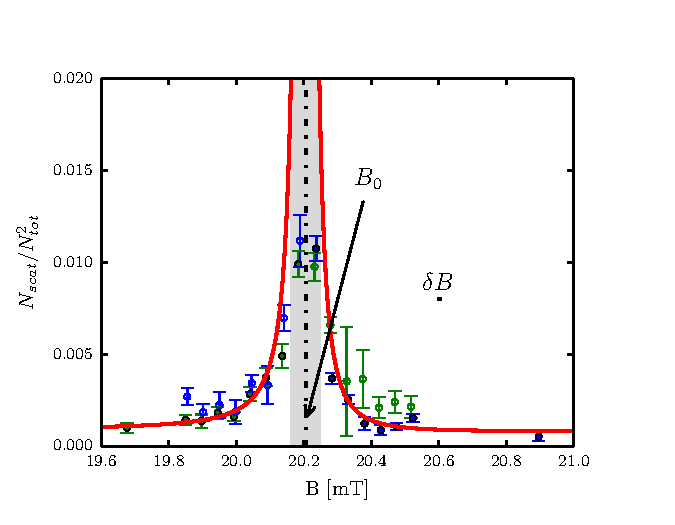
\includegraphics{figure11.pdf}
\caption{Normalized scattered population plotted versus bias field $B$. Green dots represent data taken coming from below the resonance, and blue dots represent the data taken coming from above the resonance. The red curve depicts the best fit, where data coming from above the resonance was used above the resonance and data coming from below the resonance was used below the resonance to create the fit. The regime where the scattering length is likely large enough for the atoms to behave hydrodynamically is shaded in gray. Data points in that region were not used in the fit, as there the assumption $\sigma\rho\ll1$, where $\rho$ is the atom number per unit area, is no longer valid. Values for the resonant field $B_0$ from literature and as found in this work are indicated.    }  
\label{fig:fittedFractions}
\end{figure}
\section{Conclusion}
We studied the effects of recoil-induced detuning effects on absorption images and found an optimal imaging time of $\approx40$ \us{} for \K{} atoms for noise minimization after corrections. We use these results to observe s-wave scattering halos of the Fermi gas around the Feshbach resonance and directly verify the resonance location and width. Our analysis can be used in any absorption imaging application where signal to noise minimization is critical. We performed a new kind of measurement of the resonant magnetic field and width of a Feshbach resonance. 
\section*{Acknowledgments}
We thank Marcell Gall for helpful discussions. This work was partially supported by the ARO’s Atomtronics MURI, by the
AFOSR’s Quantum Matter MURI, NIST, and the NSF through the PFC at the JQI. B.K.S. is
a NIST-NRC Postdoctoral Research Associate. L.M.A. was supported by the NSF GRFP.

\section*{References}
\bibliography{refs}{}
\bibliographystyle{plain}

\end{document}

